\chapter{Introduction}\label{ch:intro}

%-----------------------------------
\section{Problem Statement}
The \ac{UAS} has evolved tremendously over the past decade.  Miniature autopilots have gotten smaller and cheaper with more sensitive and redundant sensor packages largely due to the cellular phone industry accelerating \ac{MEMS} technology.  The ability to manufacture these autonomous systems at fractions of the cost enables the advancement in multiple cooperative UAV applications including swarming capability.  This ability to mass-produce large quantities of \ac{UAS}'s poses an interesting challenge.  Even though the price has gone down and the performance has gone up, there still exists a significant amount of man-hours dedicated to sensor calibration and autopilot control law configuration and tuning for optimal performance.  

The \ac{DoD} conducted an analysis of the role of autonomy, which outlined technology gaps and predicted advancements required to meet the growing performance demands \cite{dodroadmap}.  The study amplifies the fact that autonomy is a challenging field and that it is arguably in its infancy.  The roadmap attempts to guide decision makers in ensuring capitalization of under-utilized technology and succinct awareness of technical challenges limiting the current state of the art.  Figure~\ref{fig:dod_roadmap} outlines these elements at increasing scope of control comprised of various technology portfolios.  
\begin{figure}[h!]
 \centering
  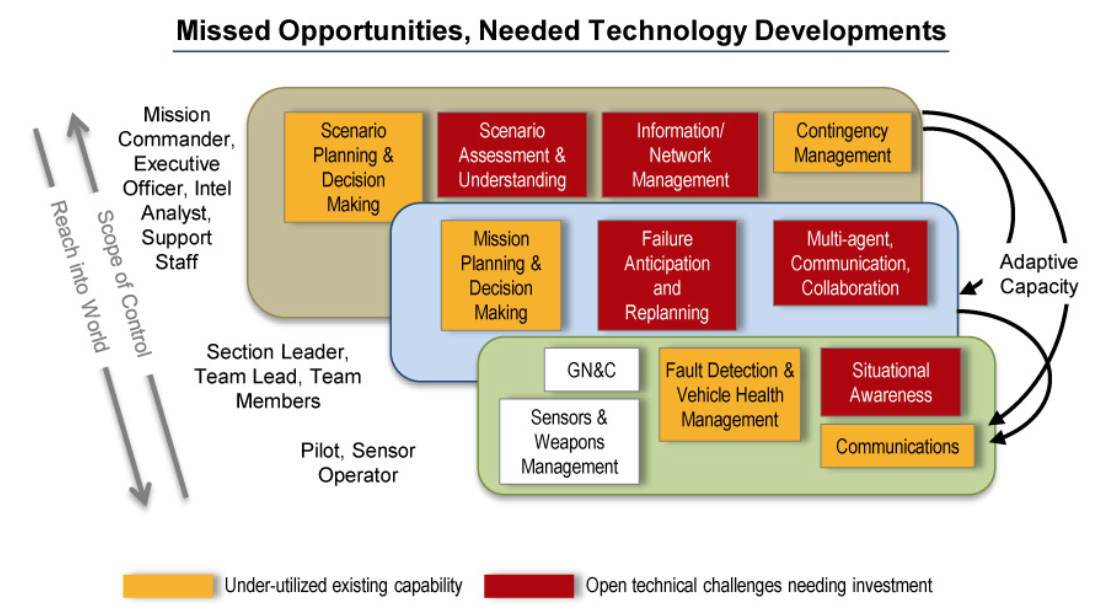
\includegraphics[width=1.0\textwidth]{DOD_roadmap.png}
  \caption{DoD Autonomy Roadmap \cite{dodroadmap}}
  \label{fig:dod_roadmap}
\end{figure}
The language referenced in the roadmap often recommends that machine learning and/or artificial intelligence is needed for elements such as "Fault Detection."  On the lowest level, the roadmap annotates the use of \ac{GNC} as neither needing improvement or current technology being underutilized.  An in-depth look at the current state of the art with respect to \ac{GNC} reveals that \ac{GNC} is still very costly and arguably antiquated.  Research of adaptive control as applied to \ac{GNC} offers new strategies offering improved performance and future reduced cost.

\ac{UAS} avionics have drastically improved over the past decade, but the fundamental control law algorithms have not changed.  The \ac{PID} architecture found its origin in automatic ship steering applications in 1922 \cite{minorsky1922pid}.  Conventional control law architectures for \ac{UAS}'s predominately still use \ac{PID} controllers.  Their architecture offers a well understood and predictable behavior for the class of linear systems.  For this reason, it is well suited for the aviation application.  The detriment of \ac{PID} control is that its application is mostly constrained by its use on a linear plant and most aerospace applications are non-linear and time varying.   An aircraft's control authority that increases proportionally to dynamic pressure is one example of significant changes in aerodynamic non-linear control behavior.  In this case, the \ac{PID} controller's robustness to changes in velocity and/or density altitude is not guaranteed and for most aircraft has to be delicately handled with lookup tables produced from hours of flight test for given configurations.

Tuning the six to ten conventional \ac{PID} controllers for one airframe is not a trivial task.  Swarming systems often will utilize the same airframe assembled by the same manufacturer, and all aircraft still require a tedious quality assurance check.  Physical aspects of the airframes such as \ac{CG}, control surface deflection/calibration/speed, and airframe alignment all can drastically vary within the same delivered batch of airframes.  Additionally, these miniature \ac{UAS}'s experience hard landings, crashes, and/or damage in transportation, which all can affect aerodynamic handling qualities.  In summary, conventional control laws require a moderate to high level of expertise in design and require significant man-hours to tune properly for every airframe even if identical.  








